%%%%%%%%%%%%%%%%%%%%%%%%%%%%%%%%%%%%%%%%%
% Arsclassica Article
% LaTeX Template
% Version 1.1 (10/6/14)
%
% This template has been downloaded from:
% http://www.LaTeXTemplates.com
%
% Original author:
% Lorenzo Pantieri (http://www.lorenzopantieri.net) with extensive modifications by:
% Vel (vel@latextemplates.com)
%
% License:
% CC BY-NC-SA 3.0 (http://creativecommons.org/licenses/by-nc-sa/3.0/)
%
%%%%%%%%%%%%%%%%%%%%%%%%%%%%%%%%%%%%%%%%%

%----------------------------------------------------------------------------------------
%	PACKAGES AND OTHER DOCUMENT CONFIGURATIONS
%----------------------------------------------------------------------------------------

\documentclass[
10pt, % Main document font size
letterpaper, % Paper type, use 'letterpaper' for US Letter paper
oneside, % One page layout (no page indentation)
%twoside, % Two page layout (page indentation for binding and different headers)
headinclude,footinclude, % Extra spacing for the header and footer
BCOR5mm, % Binding correction
]{scrartcl}

%%%%%%%%%%%%%%%%%%%%%%%%%%%%%%%%%%%%%%%%%
% Arsclassica Article
% Structure Specification File
%
% This file has been downloaded from:
% http://www.LaTeXTemplates.com
%
% Original author:
% Lorenzo Pantieri (http://www.lorenzopantieri.net) with extensive modifications by:
% Vel (vel@latextemplates.com)
%
% License:
% CC BY-NC-SA 3.0 (http://creativecommons.org/licenses/by-nc-sa/3.0/)
%
%%%%%%%%%%%%%%%%%%%%%%%%%%%%%%%%%%%%%%%%%

%----------------------------------------------------------------------------------------
%	REQUIRED PACKAGES
%----------------------------------------------------------------------------------------

\usepackage[
nochapters, % Turn off chapters since this is an article        
beramono, % Use the Bera Mono font for monospaced text (\texttt)
eulermath,% Use the Euler font for mathematics
pdfspacing, % Makes use of pdftex’ letter spacing capabilities via the microtype package
dottedtoc % Dotted lines leading to the page numbers in the table of contents
]{classicthesis} % The layout is based on the Classic Thesis style

\usepackage{arsclassica} % Modifies the Classic Thesis package

\usepackage[T1]{fontenc} % Use 8-bit encoding that has 256 glyphs

\usepackage[utf8]{inputenc} % Required for including letters with accents

\usepackage{graphicx} % Required for including images
\graphicspath{{Figures/}} % Set the default folder for images

\usepackage{enumitem} % Required for manipulating the whitespace between and within lists

\usepackage{lipsum} % Used for inserting dummy 'Lorem ipsum' text into the template

\usepackage{subfig} % Required for creating figures with multiple parts (subfigures)

\usepackage{amsmath,amssymb,amsthm} % For including math equations, theorems, symbols, etc

\usepackage{varioref} % More descriptive referencing

%----------------------------------------------------------------------------------------
%	THEOREM STYLES
%---------------------------------------------------------------------------------------

\theoremstyle{definition} % Define theorem styles here based on the definition style (used for definitions and examples)
\newtheorem{definition}{Definition}

\theoremstyle{plain} % Define theorem styles here based on the plain style (used for theorems, lemmas, propositions)
\newtheorem{theorem}{Theorem}

\theoremstyle{remark} % Define theorem styles here based on the remark style (used for remarks and notes)

%----------------------------------------------------------------------------------------
%	HYPERLINKS
%---------------------------------------------------------------------------------------

\hypersetup{
%draft, % Uncomment to remove all links (useful for printing in black and white)
colorlinks=true, breaklinks=true, bookmarks=true,bookmarksnumbered,
urlcolor=webbrown, linkcolor=RoyalBlue, citecolor=webgreen, % Link colors
pdftitle={}, % PDF title
pdfauthor={\textcopyright}, % PDF Author
pdfsubject={}, % PDF Subject
pdfkeywords={}, % PDF Keywords
pdfcreator={pdfLaTeX}, % PDF Creator
pdfproducer={LaTeX with hyperref and ClassicThesis} % PDF producer
} % Include the structure.tex file which specified the document structure and layout

\hyphenation{Fortran hy-phen-ation} % Specify custom hyphenation points in words with dashes where you would like hyphenation to occur, or alternatively, don't put any dashes in a word to stop hyphenation altogether

%----------------------------------------------------------------------------------------
%	TITLE AND AUTHOR(S)
%----------------------------------------------------------------------------------------

\title{\normalfont\spacedallcaps{Radiative Effects of Increasing Arctic Shrub Density on Seasonal Snowpack: Lessons from a Toy Energy Balance Model}} % The article title

\author{\spacedlowsmallcaps{Ian Bolliger}} % The article author(s) - author affiliations need to be specified in the AUTHOR AFFILIATIONS block

\date{} % An optional date to appear under the author(s)

%----------------------------------------------------------------------------------------

\begin{document}

%----------------------------------------------------------------------------------------
%	HEADERS
%----------------------------------------------------------------------------------------

\renewcommand{\sectionmark}[1]{\markright{\spacedlowsmallcaps{#1}}} % The header for all pages (oneside) or for even pages (twoside)
%\renewcommand{\subsectionmark}[1]{\markright{\thesubsection~#1}} % Uncomment when using the twoside option - this modifies the header on odd pages
\lehead{\mbox{\llap{\small\thepage\kern1em\color{halfgray} \vline}\color{halfgray}\hspace{0.5em}\rightmark\hfil}} % The header style

\pagestyle{scrheadings} % Enable the headers specified in this block

%----------------------------------------------------------------------------------------
%	TABLE OF CONTENTS & LISTS OF FIGURES AND TABLES
%----------------------------------------------------------------------------------------

\maketitle % Print the title/author/date block

\setcounter{tocdepth}{2} % Set the depth of the table of contents to show sections and subsections only

\tableofcontents % Print the table of contents


%----------------------------------------------------------------------------------------
%	ABSTRACT
%----------------------------------------------------------------------------------------

\section{Abstract/Introduction}

Observations of arctic shrub expansion and "greening" over the last several decades \cite{epstein_recent_2013, walker_environment_2012,elmendorf_plot-scale_2012} have led to numerous model- and field-based calculations of the net forcings and feedbacks associated with this phenomenon \cite{juszak_arctic_2014, swann_changes_2010, swann_mid-latitude_2012, bonfils_influence_2012}. The majority of these studies look at regional or global scale effects, via the use of upscaling and/or earth system models, targeting the effects on albedo, evapotranspiration, and soil temperature. One understudied potential feedback of these impacts is a change in spring snowpack ablation rate due to changing net radiative flux. This flux change is governed by two competing impacts of shrub cover: shading in the shortwave and insulation in the long wave. Here I adapt a simple canopy energy balance model \cite{mahat_canopy_2012} developed for use in spatially distributed snowmelt forecasts to the arctic environment. I first examine the tradeoffs between solar shading and longwave insulation that are introduced by shrub cover for various combinations of leaf area index (LAI) and solar zenith angle ($\theta_s$). I find that sparse shrub cover increases the net radiative flux into the snowpack over a shrub-free snowpack during low-inolation conditions in the arctic but that denser shrub cover has the opposite effect. At average and above-average insolation conditions during snowmelt season, shrub cover virtually always has a net shading effect. I also find that the negative marginal impact of increased shrub cover at low-shrub density is magnified at higher zenith angles (lower sun elevation). Next, I examine the net daily radiative flux impact of shrub cover at various LAI levels, integrating the flux as the sun traverses a typical spring/summer path in the arctic sky. I find that the net impact of increasing shrub density during snowmelt season at a latitude of 65N is one of decreasing snowpack radiative influx, as expected given the earlier results. The magnitude of the effect appears to asymptote around an LAI of 4, corresponding to a -2 kWh/day decrease in net influx.

There are two basic ways that shrub density can increase: Either by expanding to previously shrub-free areas (shrub expansion) or increasing density in already populated zones (shrub infill). The results of this toy model suggest that the strongest radiative effect on snowpack of a marginal increase in shrub density will be experienced at low densities, or in other words, in the shrub expansion scenario. The model suggests that the radiative effects will slow as LAI within a region grows through shrub infill. The non-linear relationship between shrub cover and snowpack radiative flux and the effect modification of zenith angle both have implications for the timing and duration of ablation periods, which can in turn control the timing and magnitude of vegetative production from grasses and other sub-snowpack vegetation. Understanding the effect of shrub cover on snowmelt can thus help to constrain estimates on the regional and global climate impacts of the phenomenon of arctic vegetation expansion.

 
%----------------------------------------------------------------------------------------
%	METHODS
%----------------------------------------------------------------------------------------

\section{Data and Methods}

To evaluate the implications of shrub expansion and infill on the net radiative flux of a sub-canopy snowpack, I adapted the simplified model from Mahat and Tarboton (2012) \cite{mahat_canopy_2012}. For full model details, one can read their thorough paper. Here I will simply briefly discuss the assumptions made by the model and its associated limitations. Next, I will describe the two ways in which I expanded upon the model for the purposes of measuring change in snowpack net daily radiative flux attributable to shrub expansion and infill.

%----------------------------------------------------------------------------------------
\subsection{Mahat and Tarboton (2012) Model}


The model solves analytically a system of differential equations describing the attenuation of incident radiation on a homogeneous canopy layer. It treats direct and diffuse light separately and separately models upward and downward radiation streams. It begins with Beer's law for the inicident light attenuation and adds treatment of 2 additional behaviors: (a) multiple scattering within the canopy, and (b) multiple reflections between canopy and snowpack. It treats solar and thermal infrared (IR) radiation as two distinct bands and assumes near perfect absorption of longwave radiation by both canopy and snowpack. Furthermore, it does not include an atmospheric layer, but rather treats it as a constant source/sink of IR radiation. Thus, the impacts of the canopy growth on atmospheric longwave radiation via temperature change is ignored. Despite its limitations, the simplicity of this conceptual model allows for its use in situations where few precise atmospheric and biological parameters are known. In the case of this study, in which I seek to develop high-level intuition about the relationship between shrub cover and snowmelt, such parameters are indeed too precise for inclusion in the analysis.

\subsection{Model Expansion}
First I separate daylight hours, in which the radiative influence of diffuse light is constant and that of direct light depends on $\theta_s$, from nighttime hours, in which there is no shortwave flux. Second, I develop a method for integrating over a full 24 hours of insolation, during which the sun rises, traverses a path of varying $\theta_s$ and sets.

\subsubsection{Separation of Day and Night Regimes} \label{typo}
This process is a necessary precursor to accurately integrating radiative flux over 24 hours. With regard to thermal radiation, it allows the model to alter the magnitude of longwave sources at night based on temperature changes. Simultaneously, it allows for a reasonable representation of $\theta_s(t)$ (see section \ref{integ}). This, in turn, allows me to represent $Q_sn(t)$, the net radiative flux into the snowpack as a function of time.

In both regimes (day and night), longwave flux proceeds in the same manner. These fluxes are represented in the model via the following equations, adopted from Mahat and Tarboton (2012):

\begin{align}
Q_{snl} = f_{sa}Q_{la} - Q_{ls} + f_{ss}Q_{ls} + f_{sc}Q_{lc} \\
Q_{cnl} = f_{ca}Q_{la} + f_{cs}Q_{ls} + f_{cc}Q_{lc} - 2Q_{lc} \\
Q_{rnl} = f_{aa}Q_{la} + f_{as}Q_{ls} + f_{ac}Q_{lc} - Q_{la} \text{\footnotemark}
\end{align}
\footnotetext{In Mahat and Tarboton, this last term is $+Q_{lc}$ but I believe this to be a typo. Model results confirm this assumption (see section \ref{valid})}

where $f_{ni}$ refers to the fraction of radiation emitted from source $i$ absorbed at sink $n$ and $Q_{li}$ refers to the longwave radiation emitted from layer $i$. The fractions can be approximated via the following equations, again from Mahat and Tarboton:

\begin{align}
	f_{sa} = \epsilon_s \tau_d ,\, f_{ca} = (1-\tau_d)\epsilon_c + \tau_d(1-\epsilon_s) ,\, f_{aa} = (1-\tau_d)(1-\epsilon_c) \\
	f_{ss} = (1-\tau_d)(1-\epsilon_c) ,\, f_{cs} = (1-\tau_d)\epsilon_c ,\, f_{as} = \tau_d \\
	f{sc} = \epsilon_s ,\, f_{cc} = (1- \tau_d)(1 - \epsilon_s)\epsilon_c ,\, f_{ac} = \tau_d(1-\epsilon_s)
\end{align}

where the subscripts $a$, $s$, and $c$ apply to the atmosphere, snow, and canopy, respectively, and $\tau_d$ describes the calculated transmissivity of the canopy layer. The factor $(1-\tau_d)$ accounts for the fraction of the canopy exposed \ref{mahat_canopy_2012}. These equations ignore the component of radiative transfer due to multiple reflections. The high emissivities of both snow and plants (~.98 \cite{bonan_biophysical_1991}) cause the radiation intensity to be reduced by two orders of magnitude with each reflection. Thus, this ignored component can be assumed to be negligible. The values of $f$ do not change across the day/night transition, but the thermal radiation emitted by each layer ($Q$) does due to the change in ambient air temperature. I specify one daytime and one nighttime air temperature, based on the monthly mean high and low temperatures in the CDC Derived NCEP Reanalysis Products Surface Flux data set \cite{us_department_of_commerce_esrl_????}. Within the reanalysis data set, I chose a location in the Seward Peninsula (65N, 165E) and averaged over May and June, the typical months of snowpack ablation. Because shrub temperatures are not easily available, my model assumes equilibrium between canopy and air temperatures. However, this is easily adjusted if further information on the canopy-atmosphere temperature gradient is obtained. Since the snowpack is in melt phase, $T_s$ is assumed to be at a constant $0^o$C.

\subsubsection{Integration of radiative flux over 24 hours} \label{integ}
Once the day and night distinction was made, I was able to develop a simple method for integrating the flux throughout the day as the sun traversed the horizon and its zenith angle changed. The top-of-atmosphere (TOA) mean daily insolation was calculated via a module of the climlab Python package developed by Brian Rose\footnote{This software is freely available under MIT License at github.com/brian-rose}. This module calculates zonal insolation on a given day, which, in the case of this analysis, was chosen as June 1. This day lies roughly in the middle of the arctic snowmelt period. To avoid underestimating the daytime insolation, this number was scaled up by a factor of $\frac{24}{d}$, where $d$ is the number of daylight hours for a given latitude and time of year.

\begin{figure}
\centering 
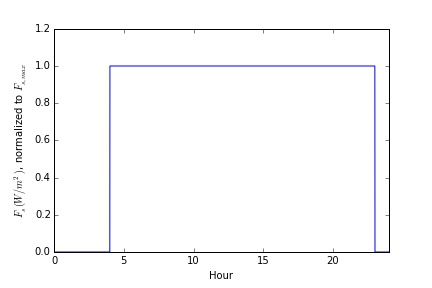
\includegraphics[width=0.75\columnwidth]{solar_assumption} 
\caption{A visualization of the simplified incoming solar radiation used in the model.}% The text in the square bracket is the caption for the list of figures while the text in the curly brackets is the figure caption
\label{fig:solar} 
\end{figure}

The atmospheric attenuation of this TOA insolation was calculated following Mahat and Tarboton (2012) such that on clear days $Q_0 = .75Q_{TOA}$, while on days with full cloud cover $Q_0 = .25Q_{TOA}$, where $Q_0$ is the incoming solar radiation at the top of the canopy. A linear extrapolation governs partial cloud cover days. For this analysis, only clear skies were analyzed; however, the model was developed such that it is easily capable of handling a varying cloud cover. As the above equation implies, for this simple analysis I assumed that the incoming solar flux at the canopy was constant throughout the day (i.e. the relationship seen in Figure \ref{fig:solar graph}). With more time, a curve could easily be developed to more accurately depict the decreased surface-level insolation at early and late daytime hours and increased insolation close to solar noon. This could be parameterized by allowing the atmospheric attenuation and/or $Q_TOA$ to vary over the course of the day. However, even with the assumption of constant daytime canopy-level insolation, the solar zenith angle still played a large role in affecting the snowpack net radiative influx by altering the effective depth of the canopy and thus the transmissivity of the canopy for direct radiation (Figure \ref{fig:heatmap}).

Due to this strong relationship between $\theta_s$ and snowpack net radiative influx, I modeled this parameter as a function of time-of-day prior to integrating over the course of an entire day to obtain daily flux values. I represented this function in the following way:

\begin{equation} \label{zen_func} E(E_{max},t,t_{rise},t_{set}) = arctan(tan(E{max}sin(\frac{(t-t_{rise})\pi}{t_{set}-t_{rise}}) \end{equation}

This formula is derived from the relationships seen in Figure \ref{fig:zen_diag}. Since the distance to the horizon-line, $D$, does not change, we can relate the height of the sun $h$ to the angular elevation $E$

\begin{equation} \label{sub_h} h = tan(E)D \end{equation}

The rising and setting of the sun can be represented by a half-period of a sine function with full period equal to twice the number of daylight hours.

$$h = h_{max} \times sin(2\pi \frac{t}{2d})$$

where $d$ is the total number of daylight hours. Substituting for $h$ with Equation \ref{sub_h} and dividing by $D$ gives us the derived relationship (Equation \ref{zen_func}). $\theta_s$ is simply $1-E$.

Once this relationship was defined, I utilized the function for $\theta_s$ in the model derived from Mahat and Tarboton (2012) and integrated over time from sunrise to sunset. After adding in the nightime longwave flux, I arrived at the daily snowpack net radiative flux.

\begin{figure}
\centering 
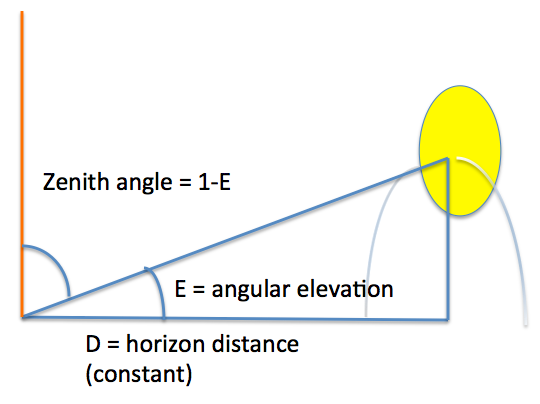
\includegraphics[width=0.75\columnwidth]{zenith_diag} 
\caption{A diagram of the relationship of $\theta_s$ to the path of the sun in a given day}
\label{fig:zen_diag} 
\end{figure}


%----------------------------------------------------------------------------------------
%	RESULTS AND DISCUSSION
%----------------------------------------------------------------------------------------

\section{Results and Discussion}

\subsection{Model Face Validity} \label{valid}
I performed several simple face validity checks prior to interpreting any results in order to confirm that the model I had coded was both reasonable and representative of the relationships I had obtained from Mahat and Tarboton (2012). First, I sought to reproduce a figure that related canopy shortwave transmittance, $\tau$ to zenith angle, $\theta_s$. The resultant plot (Figure \ref{fig:t_z}) did indeed match that of the original paper. Furthermore, it shows the relative importance of accounting for multiple scattering within the canopy at high and low zenith angles. For a sun that's directly overhead, multiple scattering significantly increases the transmitted direct radiation, while in high-$\theta_s$ regimes, the scattering impact on transmittance is much lower.

\begin{figure}
\centering 
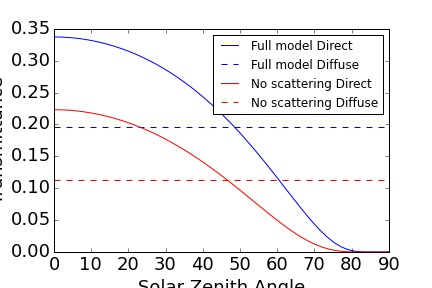
\includegraphics[width=0.75\columnwidth]{transmittance} 
\caption{A reproduction of a figure from Mahat and Tarboton suggests that the underlying model I coded accurately implements the equations obtained from that paper. The figure relates canopy transmittance (the ratio of intensity of a single beam leaving the canopy to its intensity entering) to solar zenith angle $\theta_s$. The "No scattering" curves refer to the baseline model proposed by Mahat and Tarboton, which is purely an implementation of Beer's Law.}
\label{fig:t_z} 
\end{figure}

In my formulation of the longwave radiative transfer equations, I deviated from those described in Mahat and Tarboton (2012) due to my assumption that their manuscript contained a typo (see Section \ref{typo}). Thus, I sought to verify face validity of the longwave equations by summing the net atmospheric, canopy, and snow surface longwave fluxes for various parameter settings. As expected, all scenarios yielded no net flux from the system. This is intuitively valid, as there are no external sources or sinks to our snow-surface/canopy/atmosphere system.

Once face validity was established I began two distinct analyses. The first centered on establishing the relationship of snowpack net radiative flux to shrub cover leaf area index (LAI) and $\theta_s$. The second estimated the impact on daily snowpack net radiative flux of shrub cover for various LAI values at a typical latitude where shrub expansion and infill are occurring.

\subsection{Snowpack radiative flux, LAI, and $\theta_s$}
The impacts of snowpack shading (in the shortwave) and insulation (in the longwave) are competing with respect to the net radiative flux into or out of the snowpack. Thus, it is unclear whether increasing the shrub density and/or coverage increase or decrease this net flux. To examine this relationship, I parameterized my model based on mean May-June temperatures and mean June 1 insolation. I then allowed the zenith angle and LAI to vary from $0$ to $90^oC$ and $0.0 to 3.0$, respectively. To examine how this relationship played out at different canopy-level solar insolation values, I re-ran the model at $1/2x$ and $2x$ the mean June 1 insolation. The results are seen in Figure \ref{heatmaps}.

\begin{figure}
\centering 
\makebox[\textwidth][c]{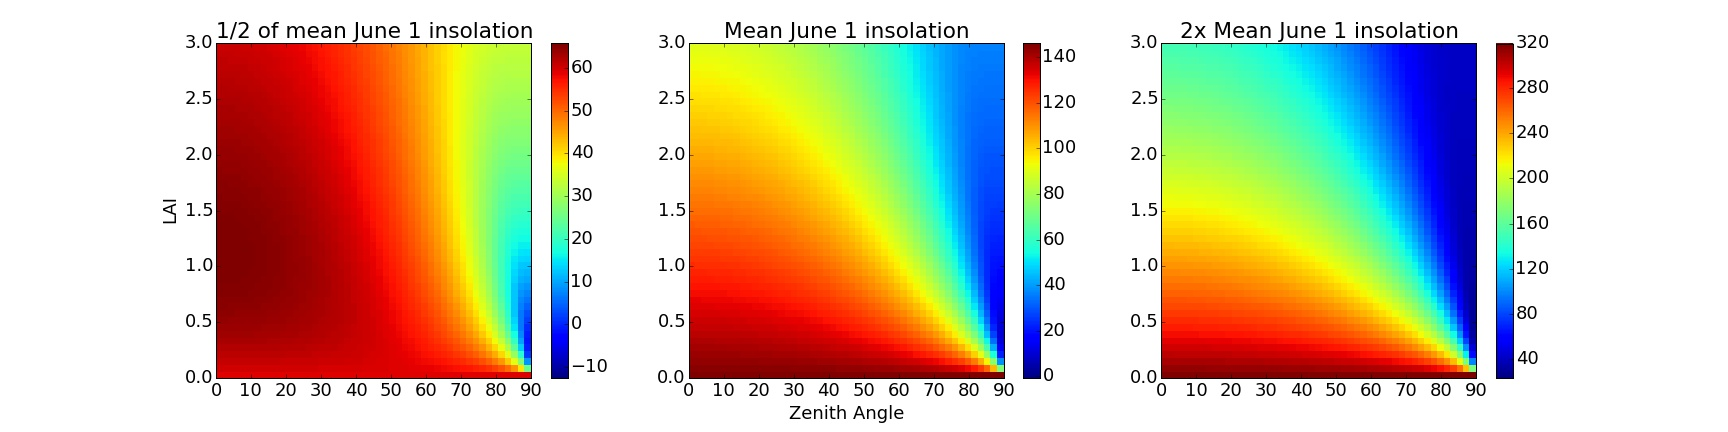
\includegraphics[width=2\columnwidth]{colormaps} }
\caption{Heatmaps of the net radiative flux into the snowpack for a given LAI and $\theta_x$. The parameters used for these model runs are representative of late-May/early-June conditions on the Seward Peninsula at 65N, except for the mean insolation. The left-most figure uses one-half of the mean May-June insolation, the center figure uses the mean itself, while the right-most figure uses twice the mean.}
\label{fig:heatmaps} 
\end{figure}

It is clear from the appearance of these figures that the effect of increasing shrub density is non-linear and depends strongly on the mean top-of-canopy insolation. When top-of-canopy insulation is low (as in the left heatmap), and when zenith angle is also low, low-density shrubs increase the net snowpack radiative influx due to an insulating effect. However, when the shrub cover becomes denser, the effect is reversed. This indicates that at higher LAI values, shading dominates insulation when the sun is high in the sky but weak. At higher zenith values (i.e. sun low in the sky), this relationship is reversed. In other words, low-density shrubs decrease net snowpack influx while higher density shrubs increase it. This affect can also be understood intuitively. When the sun is very low in the sky, the effective canopy depth is quite high. Thus, just a low density of leaves will almost entirely block insulation from reaching the underlying snowpack. As the canopy becomes more and more dense, there is no sunlight left to shade from yet the insolation effect is allowed to increase.

At mean June 1 insolation, the insulation effect no longer dominates at low LAI and low $\theta_s$. In other words, adding even low density shrubs will decrease the net snowpack influx relative to a shrub-free environment. However, at high zenith angles, we see a similar relationship to the low-insolation case. That is, a rapid decrease in radiative influx with low-density shrubs and then a slow increase as the shrubs become denser. It should be noted, however, that this increase does not start to occur until an LAI of roughly $1.5$. While the range of LAI values assumed in this analysis was intentionally large due to the desire to explore the extreme values of a potential parameter space, maximum arctic shrub LAI values are, in reality, somewhere in the neighborhood of 1-2 \cite{chen_relating_2009}. Thus, the effect of increasing shrub infill and/or expansion on mid-snowmelt season radiative influx is a negative one in almost all cases. This has implications for considering feedbacks to shrub growth. If the presence of shrubs were to extend the snowmelt duration, it would delay the appearance of grasses and other sub-snowpack vegetation. This would provide a negative feedback with respect to albedo and evapotranspiration, though estimating the magnitude of this feedback is beyond the scope of this analysis.

The 2x mean June 1 insolation values are largely unrealistic for snowmelt season and do not display any significantly surprising behavior. The heatmap is similar in appearance to the mean heatmap, though without the decrease in net influx seen at higher LAI and higher zenith angle values.

\subsection{Impact of shrub coverage on daily snowpack radiative influx}
The results of the above analysis led me to wonder at the net daily affect of shrub cover as the sun traversed from high $\theta_s$ to low and back to high. Applying the model described above to integrate flux over the course of a day, I obtained the results seen in Figure \ref{fig:daily_int}. In creating these figures, I chose a maximum angular sun elevation $E_max$ of $47^o$ and a daylight duration of 20.5 hours. These numbers are representative of June 1 values for the 65N zonal band \cite{us_department_of_commerce_esrl_????-1}.

\begin{figure}
\makebox[\textwidth][c]{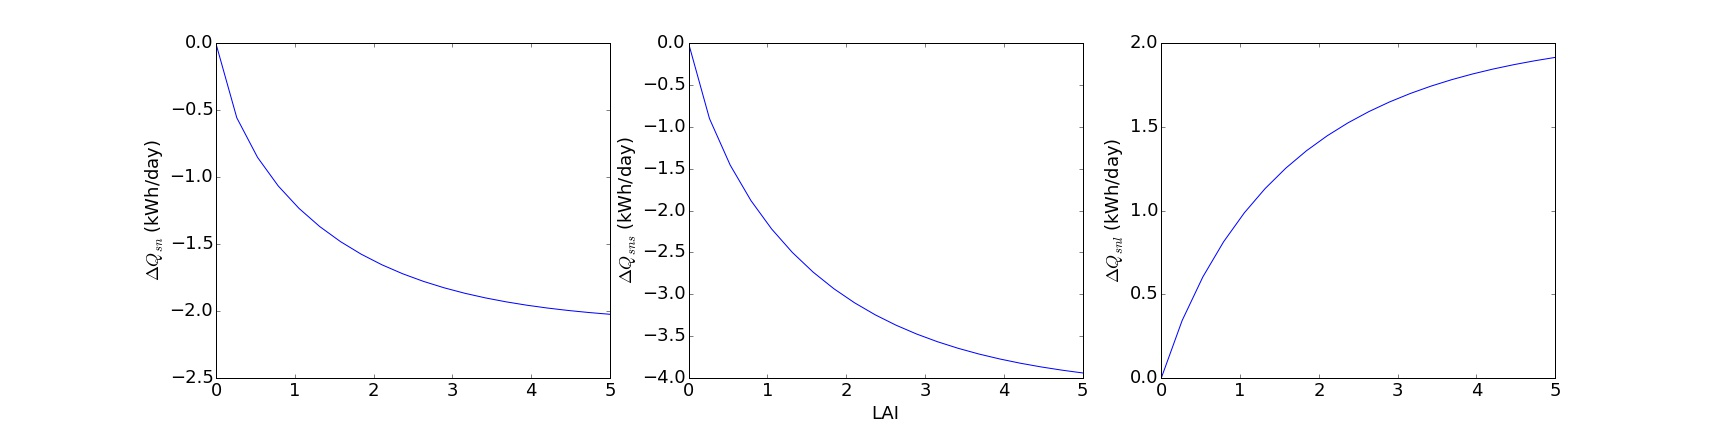
\includegraphics[width=2\columnwidth]{daily_int} }
\centering 
\caption{The effect on daily snowpack net radiative influx of increasing shrub-density for typical mid-snowmelt season air temperatures, TOA insolation values, daylight duration, and maximum zenith angle at 65N. The leftmost figure displays the effect on total net radiative influx ($Q_{sn}$), the middle figure displays the effect on shortwave influx ($Q_{sns}$), and the rightmost figure displays the effect on longwave influx ($Q_{snl}$).}
\label{fig:daily_int} 
\end{figure}

Several qualitative and quantitative aspects of this figure stand out. On the qualitative side, as expected, we see the net shortwave flux decreasing strongly with increasing LAI and the net longwave flux increasing with increasing LAI. This, again, points to the competing insulation and shading effects of shrub cover. Looking at the total change in $Q_ns$ (the left-most figure), it is clear that for this circumstance the shading effect clearly dominates. Reviewing the results seen in Figure \ref{fig:heatmaps}, this makes sense. For all zenith angles in the "Mean June 1 insolation" heatmap, we see a decreasing $Q_sn$ with increasing LAI. In the higher zenith angles, where the integrated daily flux calculation lies, we see that this decrease is especially sharp as we begin to add low-density shrubs to a shrub-free environment. Again, this rapid negative effect on snowpack radiative influx is due to the large effective canopy depth for high zenith angles. From a qualitative standpoint, this has large implications for northward Arctic vegetation expansion. As warmer weather allows for this northward migration, shrubs that rise above the snow during ablation season will have a stronger and stronger negative feedback on snowmelt due to the higher zenith angles at higher latitudes. As mentioned previously, the magnitude of this feedback is unfortunately beyond the scope of this toy model.

From a quantitative perspective, two elements of these figures stick out. First, we seem to see an asymptote of the net radiative impact at around $-2$ kWh/day, which is roughly achieved around an LAI of 4. Interestingly, this is not because the impacts of further increasing shrub density on short and longwave net fluxes approach 0. If this were the case, we would see similar asymptotes in the short- and long-wave figures. Instead, it appears that these effects begin to balance out. That is, while the rate of change in shortwave influx with respect to LAI ($\frac{dQ_{sns}}{dLAI}$) is sharp at first, it slows quickly, allowing $\frac{dQ_{snl}}{dLAI}$ to catch up. To be fair, these banded fluxes also begin to asymptote at higher shrub densities. However, it is interesting that the asymptote appears for the net flux at lower LAI values. Again, realistic arctic shrub LAI's are typically $<2$, which implies that this asymptote falls outside of the expected range. A second notable element of this figure is the magnitude of forcing. At a large but physically reasonable LAI of 1, we see a roughly 1.25 kWh/day reduction in $Q_sn$. At face value, this seems a rather large reduction as canopy-free $Q_sn$ is only around 3.3 kWh/day (model results, not pictured). However, given the high zenith angle, this significant reduction is not outright implausible. Further model development would likely shed light on whether this large magnitude is reasonable or is an artifact of this simplistic model design.

%------------------------------------------------

\section{Conclusions}
Though simple, the model described in this paper provides some valuable insight into the feedbacks of shrub expansion and infill on snowmelt in the Arctic. The broadest "zero-order" conclusion I have reached is that in virtually all plausible Arctic snowmelt-season conditions increasing shrub cover creates induces a negative forcing on snowpack net radiative influx. One might refer to this a negative feedback with respect to surface temperature, as decreasing the radiative influx to a melting snowpack will prolong its seasonal existance and delay the sharp drop in albedo associated with full melt. To expand on this relationship, the model indicates that the marginal effect of increasing shrub density at low-densities is quite strong at high solar zenith angles. Since the Arctic is characterized by such zenith angles, it appears that the initial emergence of shrubs above the snowpack (i.e. through habitat expansion) will have a greater impact than further growth within an already populated area (i.e. infill). This effect is largely due to the large effective canopy depth caused by high zenith angles. As warming temperatures drives northward shrub expansion, the canopies will experience lower and lower solar elevations, making the negative feedback of shrub growth at low-densities even stronger.

Simple models like this one can provide valuable intuition about the processes governing a complex competing-effect phenomena like the effect of shrub growth on snowmelt. This is intuition that is often difficult to glean when viewing the results of a more physically representative earth system model, for instance. However, it is important to be wary of the applicability of the results, especially with respect to absolute effect magnitudes. While I am reasonably confident in my model's ability to accurately represent the qualitative relationships described in the preceeding paragraph, I am hesitant to discuss the implications of the effect magnitudes output by the model. This is due to the many limitations of this toy approach. The list of these limitations is long and includes an assumption of equivalent canopy skin temperature and ambient air temperature, an assumption of isotropic leaf orientation, a lack of distinction between woody biomass and leaves, and a constant LAI as snow melts. Arguments could me made for why each of these assumptions would significantly affect the magnitude of the model results. Another significant limitation was the assumption of constant daytime insolation. As the sun traverses from low to high to low elevation, the top-of-canopy insolation experiences a similar sinusoidal pattern. This was not accounted for in the model and may influence the integrated daily flux results, downweighting the effects of increased effective canopy depth at low solar elevations. Implementing this variable insolation value would not be difficult with slightly more time and represents a logical next step in this model.

Beyond the scope of this energy balance model lies the full impact of shrub cover on snowmelt. This process is driven not just by radiative flux but by turbulent sensible and latent heat fluxes, heat input from rain, and conductive exchange with the ground \cite{serreze_snow_????}. Shrub expansion and infill could alter some if not all of these other processes, which would need to be accounted for to determine the full net impact of shrub cover on snowmelt timing and duration.

%----------------------------------------------------------------------------------------
%	BIBLIOGRAPHY
%----------------------------------------------------------------------------------------

\renewcommand{\refname}{\spacedlowsmallcaps{References}} % For modifying the bibliography heading

\bibliographystyle{unsrt}

\bibliography{bib} % The file containing the bibliography

%----------------------------------------------------------------------------------------

\end{document}
